\documentclass{article_saj}
\pagestyle{myheadings}
\usepackage{graphicx,saj,multicol,subeqnarray}
\usepackage{natbib}
\usepackage{float}
\usepackage{xcolor}
\usepackage{widetext}
\usepackage{url}
\usepackage{bm}
\usepackage{tikz} % for checkmark
\usepackage{pifont} % for xmark
\usepackage{amsfonts}
\usepackage{amssymb}
\usepackage{amsmath,upgreek}
\usepackage{titlesec}
\usepackage{float}
\def\tg{\mathop{\rm tg}\nolimits}
\def\arctg{\mathop{\rm arctg}\nolimits}

\def\point#1{\hbox{\setbox7=\hbox to0.6em{\hfil.\hfil}%
\setbox8=\hbox to0.5em{\hfil$^{#1}$\hfil}%
\box7\kern-0.5em\box8}}

\def\pointmin#1{\hbox{\setbox2=\hbox to0.8em{\hfil.\hfil}%
\setbox3=\hbox to0.6em{\hfil$^{#1}$\hfil}%
\box2\kern-.7em\box3}}

%for non integer numbers for years, days, hours, minutes and seconds

\def\yyy{\point{\mathrm{y}}}
\def\ddd{\point{\mathrm{d}}}
\def\hhh{\point{\mathrm{h}}}
\def\mmm{\pointmin{\mathrm{m}}\kern.15em}
\def\sss{\point{\mathrm{s}}}

%for non integer numbers for arc degrees, arc minutes and arc seconds

\def\oo{\point{\circ}}
\def\lll{\point{\prime}}
\def\uu{\point{\prime\prime}}

%for integer numbers for arc degrees, arc minutes and arc seconds

\def\OO{$^\circ$}
\def\LLL{$^\prime$}
\def\UU{$^{\prime\prime}$}
 

\titlelabel{\thetitle.\quad}
\definecolor{xlinkcolor}{cmyk}{1,0.6,0,0}
\usepackage[bookmarks=false,         % show bookmarks bar?
     pdfnewwindow=true,      % links in new window
     colorlinks=true,    % false: boxed links; true: colored links
     linkcolor=xlinkcolor,     % color of internal links
     citecolor=xlinkcolor,     % color of links to bibliography
     filecolor=xlinkcolor,  % color of file links
     urlcolor=xlinkcolor,      % color of external links
final=true
]{hyperref}

% Papertype can be "Invited Review", "Original Scientific Paper",
% "Preliminary report" or "Professional paper"

\def\papertype{\ \hfill\ Editorial}

\def\udc{52}
\setcounter{publno}{200}
\setcounter{publyear}{2020}
\setcounter{page}{1}
\setcounter{firstpage}{1}
\setcounter{lastpage}{5}

\citestyle{kluwer}%

\setcounter{footnote}{0}
\renewcommand{\thefootnote}{\fnsymbol{footnote}}

\begin{document}
\parindent=.5cm
\baselineskip=3.8truemm
\columnsep=.5truecm
%
\newenvironment{lefteqnarray}{\arraycolsep=0pt\begin{eqnarray}}
{\end{eqnarray}\protect\aftergroup\ignorespaces}
\newenvironment{lefteqnarray*}{\arraycolsep=0pt\begin{eqnarray*}}
{\end{eqnarray*}\protect\aftergroup\ignorespaces}
\newenvironment{leftsubeqnarray}{\arraycolsep=0pt\begin{subeqnarray}}
{\end{subeqnarray}\protect\aftergroup\ignorespaces}
%

% Runningtitle

\markboth{\eightrm ANÁLISIS DE RESULTADOS - TAREA 2} 
{\eightrm C. Axel }

\begin{strip}


% Title

\title{INFORME DE RESULTADOS - TAREA 2}

% Authors

\authors{C. Axel}

\vskip3mm

% Address

\address{$^1$Tecnológico de Costa Rica, Escuela de Ingeniería en Computación 
\break Inteligencia Artificial - IC6200 - Grupo 2}

% E-mail

\Email{axelchaves.r@estudiantec.cr}



\end{strip}

\tenrm

% Sections
\textbf{
Abstract-- Este informe pretende mostrar los resultados de análisis del conjunto de datos llamado \textit{Iris Flower}, el cual contiene datos relacionados a ciertas especies de flores. A su vez, se muestran distintos elementos que permiten mostrar la evaluación de dicho conjunto de datos a través del algoritmo de clasificación \textit{K-Nearest Neighbors} y las conclusiones sobre las pruebas realizadas. 
}
\section{INTRODUCCIÓN}

\indent

A continuación se presenta una investigación con el propósito de mostrar el procedimiento y análisis de la implementación del algoritmo de clasificación \textit{K-Nearest Neighbors}. En detalle, este informe contiene la ejecución del algoritmo, gráficos que permiten realizar conclusiones sobre los datos utilizados y el resultado obtenido posterior al desarrollo. 


\section{ANÁLISIS DE CARACTERÍSTICAS}

\indent

El conjunto de datos sobre el que se implementó el algoritmo corresponde a \textit{Iris Flower}. Dichos datos contienen información sobre estos tipos de flores: \textit{Iris setosa, Iris versicolor e Iris virginica} además de la longitud y anchura de sus sépalos y pétalos. 

\subsection{Longitud y Ancho Sépalos y Pétalos}

\indent
Como resultado de implementar este gráfico se puede concluir que, en la mayoría de casos, tanto el sépalo como el pétalo de las flores cuentan mayoritariamente con una longitud mayor que su ancho. De hecho, en algunos casos se supera el tamaño casi duplicando al ancho.  

\begin{figure}[H]
\centerline{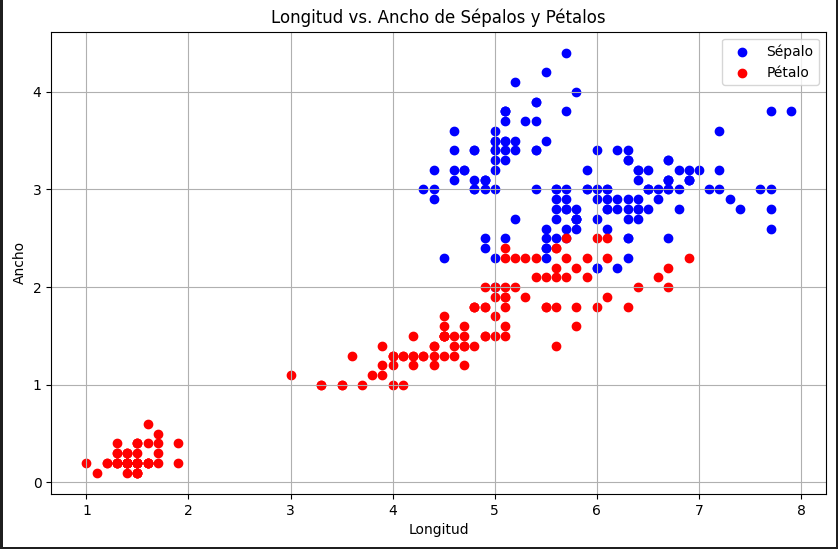
\includegraphics[width=0.8\columnwidth, keepaspectratio]{chart1.png}}
\caption{Gráfico de comparación de anchura y altura de sépalos y pétalos.}
\label{fig1}
\end{figure}


\subsection{Longitud de Pétalos vs Sépalos}

\indent

Al analizar este gráfico, se encontró que la diferencia entre el largo del pétalo y el sépalo de las flores es significativa, lo que lleva a concluir que los pétalos tienen una extensión menor, ya que existe una cantidad importante de pétalos con un tamaño menor a la longitud de los pétalos. 

\begin{figure}[H]
\centerline{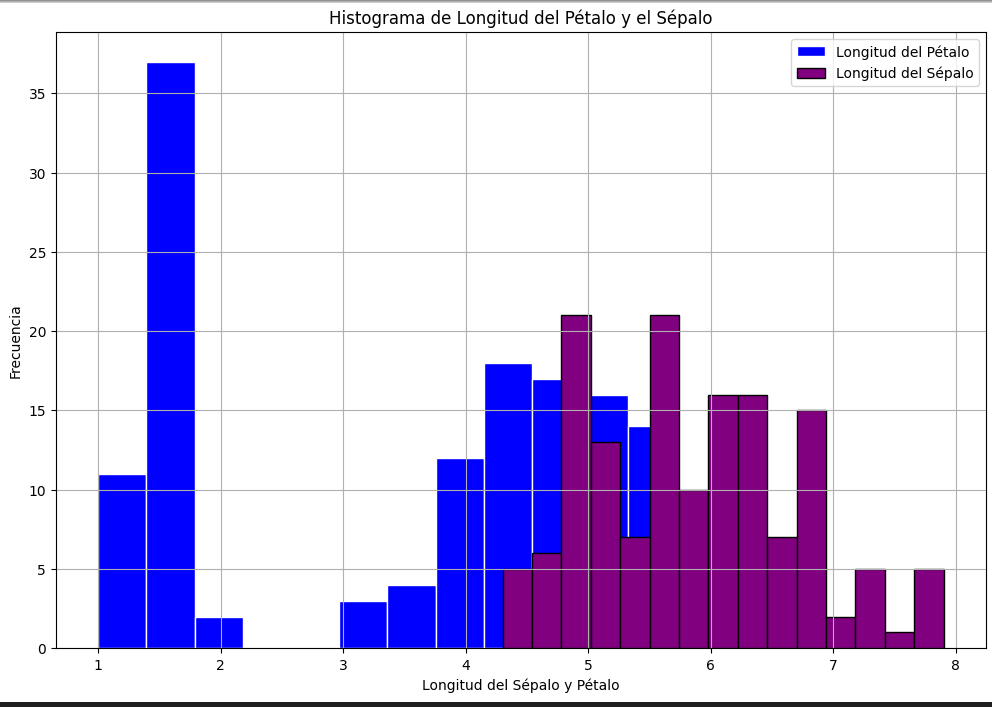
\includegraphics[width=0.6\columnwidth, keepaspectratio]{chart2.png}}
\caption{Histograma de longitud de los pétalos y los sépalos.}
\label{fig2}
\end{figure}

\subsection{Anchura de Pétalos vs Sépalos}

\indent

Con el siguiente gráfico, se encontró que los sépalos tienen un ancho descomunalmente superior a los pétalos. 

\begin{figure}[H]
\centerline{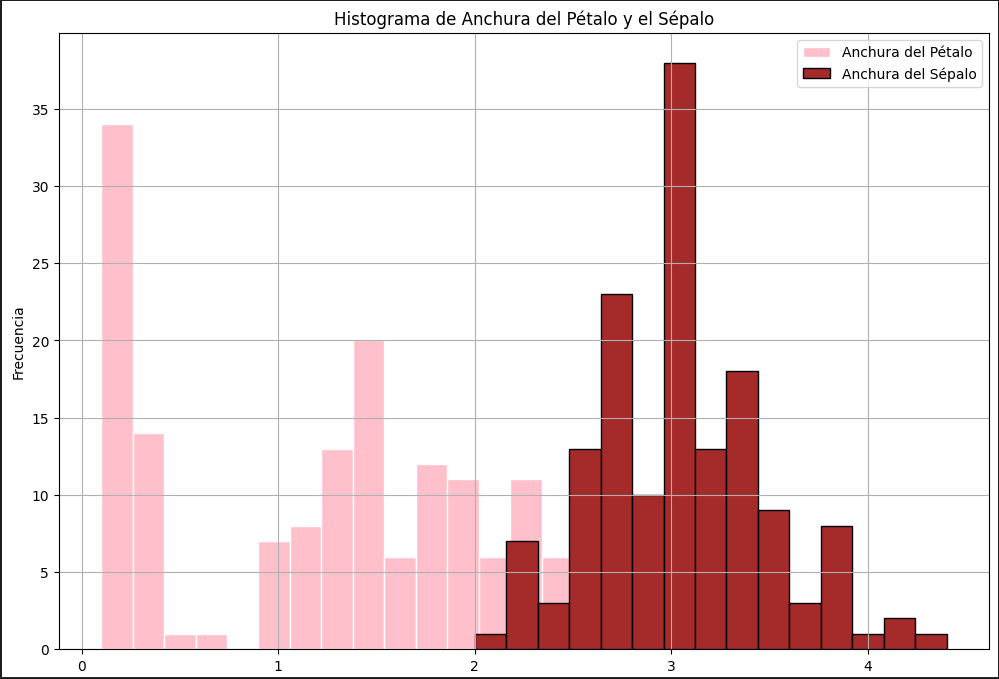
\includegraphics[width=0.8\columnwidth, keepaspectratio]{chart3.png}}
\caption{Histograma de anchura de los pétalos y los sépalos.}
\label{fig3}
\end{figure}

\subsection{Longitud del Sépalo vs Su Altura}

\indent

El gráfico implementado muestra la relación entre ancho y alto del sépalo según el tipo de flor, lo cual muestra las diferencias notables que existen según la especie.

\begin{figure}[H]
\centerline{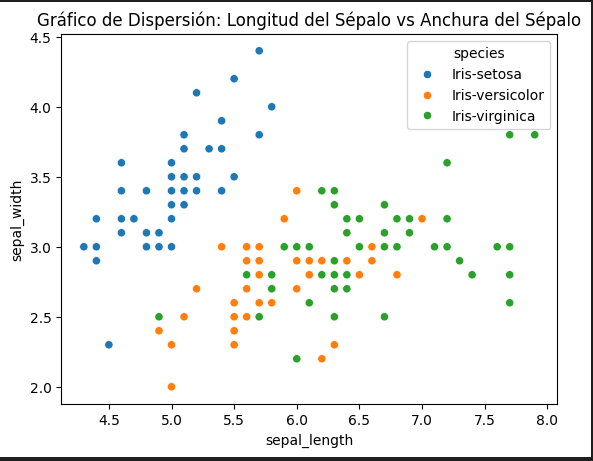
\includegraphics[width=0.8\columnwidth, keepaspectratio]{chart4.png}}
\caption{Gráfico de dispersión de la anchura y altura de los sépalos según la flor.}
\label{fig4}
\end{figure}

\subsection{Síntesis de Resultados}

\indent

Una vez mostrados los resultados del análisis, es posible sacar ciertas conclusiones. Primero, la diferencia entre las flores es notable, tanto a nivel de altura como anchura. Asimismo, la relación entre altura y anchura de los pétalos y los sépalos es muy distinta, dada la naturaleza de los datos. En síntesis, el análisis resultó enriquecedor para conocer la naturaleza de los datos y poder entrar en la etapa de aplicación del algoritmo.

\section{APLICACIÓN DE ALGORITMO KNN}

\indent

El algoritmo \textit{K-Nearest Neighbors} corresponde a uno de los algoritmos más básicos para resolver problemas de clasificación de datos. Asimismo, este es capaz de producir resultados competitivos y es fundamental en la minería de datos [1]. 
\indent

Entre los elementos fundamentales que necesita el algoritmo para funcionar están: un conjunto de datos, \textit{features} y etiquetas.

\subsection{Algoritmo Detallado}

\indent

A continuación, se muestra el código fuente del algoritmo en cuestión.

\begin{figure}[H]
\centerline{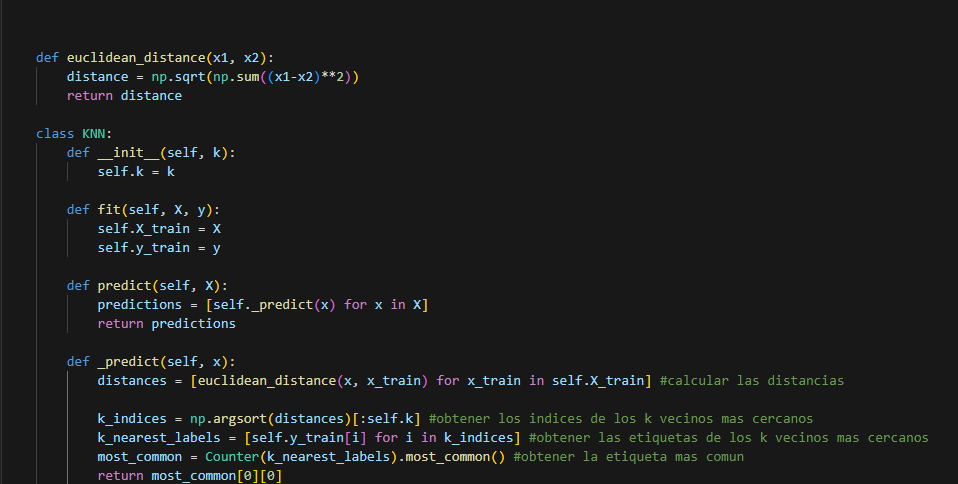
\includegraphics[width=0.8\columnwidth, keepaspectratio]{knn.png}}
\caption{Algoritmo KNN. Lenguaje de programación: Python}
\label{fig5}
\end{figure}

Brevemente, el algoritmo funciona de la siguiente manera:

\indent

Se debe inicializar el algoritmo con un número arbitario de elementos k, los cuales representan la cantidad de vecinos cercanos al punto a considerar. Además, la distancia euclídea se utiliza para  calcular las distancias entre puntos. Asimismo, se obtienen las etiquetas de los vecinos cercanos y se obtiene la etiqueta más común. 
\indent

Después de este procedimiento, el algoritmo será capaz de ajustarse al modelo de datos y realizar predicciones. 

\subsection{Procedimiento}

\indent

El procedimiento utilizado para implementar este algoritmo fue el siguiente: 

\indent

Primero, se obtiene el conjunto de datos a utilizar. En este caso, Iris.

\begin{figure}[H]
\centerline{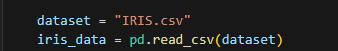
\includegraphics[width=0.8\columnwidth, keepaspectratio]{retrieveDataset.png}}
\caption{Código para obtener el conjunto de datos. Lenguaje: Python}
\label{fig6}
\end{figure}

\indent

Segundo, se obtiene el conjunto de datos y se separa para utilizar una parte para el entrenamiento y otra para realizar pruebas.

\begin{figure}[H]
\centerline{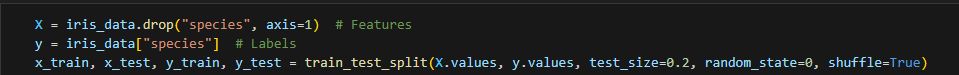
\includegraphics[width=0.8\columnwidth, keepaspectratio]{step2.png}}
\caption{Código para separar los datos. Lenguaje: Python}
\label{fig7}
\end{figure}

Tercero, se realizan pruebas con valores distintos de k con el fin de probar la precisión de este valor en el algoritmo KNN. 

\begin{figure}[H]
\centerline{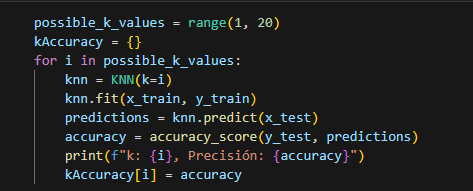
\includegraphics[width=0.8\columnwidth, keepaspectratio]{kTest.png}}
\caption{Código que implementa pruebas de algoritmo KNN. Lenguaje: Python}
\label{fig8}
\end{figure}
\subsection{Hiperparámetro del Algoritmo}
\indent

El hiperparámetro utilizado en este algoritmo corresponde a \begin{math}
    k
\end{math}, el cual es modificado manualmente para realizar pruebas que determinen el valor adecuado que debe tener para que la precisión sea lo más alta posible. En este caso, \begin{math}
    k
\end{math} corresponde a un número entero mayor o igual a 1.

\section{EVALUACIÓN DEL MODELO UTILIZADO}
\indent

Para analizar los resultados, se toma como referencia el hiperparámetro \begin{math}
    k=8
\end{math}, dado que fue uno de los valores que presenta un 100\% de precisión y es óptimo para obtener una matriz de confusión. La salida obtenida es la siguiente:

\indent


\begin{bmatrix}
11 & 0 & 0\\
0 & 13 & 0\\
0 & 0 & 6   
\end{bmatrix}

\indent

Asimismo, se muestra la relación de la precisión de las predicciones respecto al \begin{math}
    k
\end{math} utilizado.

\begin{figure}[H]
\centerline{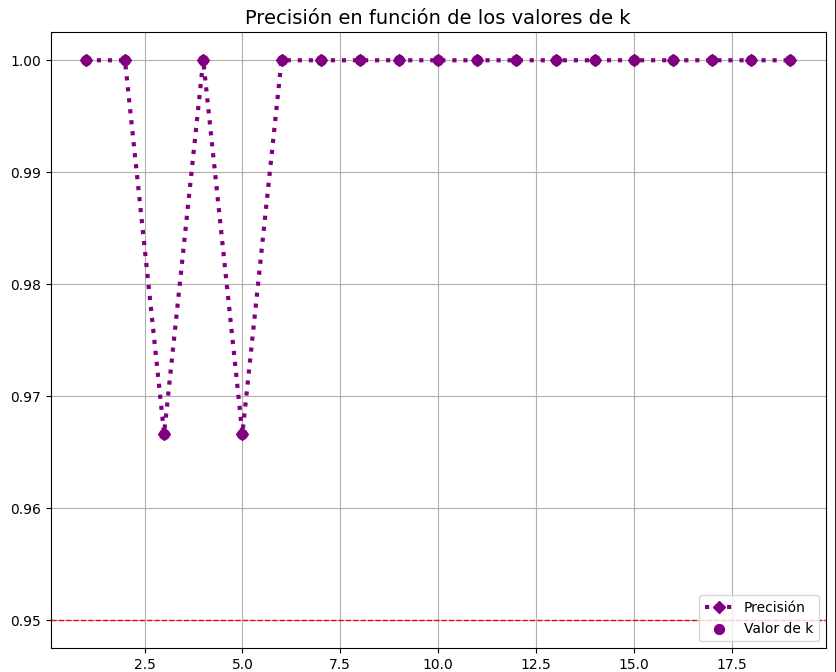
\includegraphics[width=0.8\columnwidth, keepaspectratio]{finalChart.png}}
\caption{Gráfico lineal de relación entre el k utilizado y la precisión obtenida.}
\label{fig9}
\end{figure}
\subsection{Pérdida de Precisión del Modelo}

\indent

El modelo utilizado es realmente preciso con muchos valores de \begin{math}
    k
\end{math}, sin embargo, empieza a perder su precisión con ciertos valores cuando se supera un número de \begin{math}
    k
\end{math} mayor a 50, como se muestra en el siguiente gráfico. 

\begin{figure}[H]
\centerline{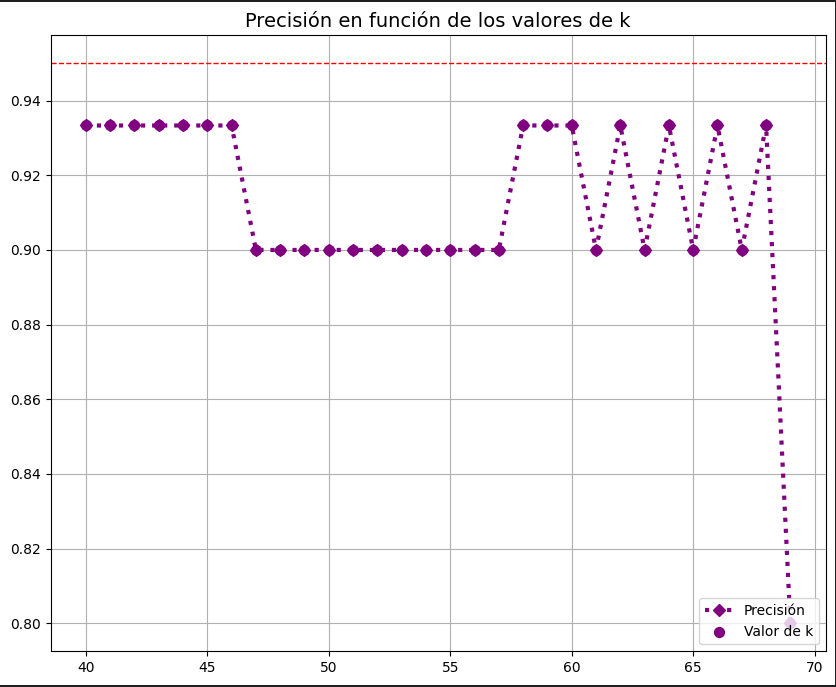
\includegraphics[width=0.8\columnwidth, keepaspectratio]{otherChart.png}}
\caption{Gráfico lineal que representa la relación de k con la precisión. Rango k = [40,70[}
\label{fig10}
\end{figure}

Entre los motivos que pueden justificar esta pérdida de precisión, es que, a pesar de que es un algoritmo simple de implementar, es sensible ante datos atípicos y puede perder su precisión al tener distancias con rangos distintos [2].

\section{CONCLUSIONES}

\indent

En base a los resultados y el análisis efectuado, es importante destacar ciertos puntos:

\indent

Primero, el algoritmo implementado presenta una diversidad de valores \begin{math}
    k
\end{math} que alcanzan una precisión perfecta.

\indent

Segundo, el conjunto de datos utilizado es relativamente pequeño, ya que alcanza los 150 elementos, lo cual favorece directamente al algoritmo KNN debido a que este tiende a perder precisión al utilizar conjuntos de datos muy grandes. 

\indent

Tercero, el análisis realizado mediante gráficos determina que existen ciertas relaciones y diferencias entre los datos que el algoritmo puede utilizar a su favor, a modo de mejorar su capacidad de predicción, lo cual ya fue corroborado mediante el ejercicio de pruebas. 

\indent

Cuarto, mediante uno de los gráficos mostrados, es posible visualizar que hay una relación lineal entre los datos, lo cual beneficia una vez más al algoritmo.

\indent

En síntesis, el algoritmo KNN fue capaz de realizar predicciones de un modelo simple. Además, la parte analítica de esta investigación fue fundamental para comprender el comportamiento del algoritmo sobre los datos utilizados. 

\section*{REFERENCIAS}
\begin{referencias}

\bibitem{leon2023}
[1]  \: M.I.A. Palacio, M.J.B. Vélez and I.M. Henao, '"Predicción de enfermedades del corazón usando el algoritmo K-Nearest Neighbors," Universidad EAFIT, Medellín.


\bibitem{montalvo2012}
[2]  \:   C.J. Madariaga Fernández, Y.O. Lao León, D.A. Curra Sosa and R. Lorenzo Martín, '"Empleo de algoritmos KNN en metodología multicriterio para la clasificación de clientes, como sustento de la planeación agregada," Retos de la Dirección, vol. 16, no. 1, pp. 178-198.
\bibitem{hernandez1975}


\end{referencias}
 


%%%%%%%%%%%%%%%%%%%%%%%%%%%%%%%%%%%%%%%%%%%%%%%%%%%%%%%%%%%%%%%%%%%%%%%%%%%%%
%                       C O M P I L I N G
% You must compile your LaTeX source text "mysource.tex" in THE following
% way:
%  pdflatex mysource
%  bibtex mysource
%  pdflatex mysource
%  pdflatex mysource
% Compiling twice is required to set all the parameters needed
% (lastpage, labels...) properly. It will also generate the mysource.bbl
% with your bibliography.
%%%%%%%%%%%%%%%%%%%%%%%%%%%%%%%%%%%%%%%%%%%%%%%%%%%%%%%%%%%%%%%%%%%%%%%%%%%%%

\end{document}
